\documentclass[12pt,a4paper]{article}
\usepackage[utf8]{inputenc} %polskie znaki
\usepackage[T1]{fontenc}	%polskie znaki
\usepackage{amsmath}		%matematyczne znaczki :3
\usepackage{enumerate}		%Dodatkowe opcje do funkcji enumerate
\usepackage{geometry} 		%Ustawianie marginesow
\usepackage{graphicx}		%Grafika
\usepackage{wrapfig}		%Grafika obok textu
\usepackage{float}			%Allows H in fugire
\usepackage{hyperref}		%Allows hyperlinks
%\pagestyle{empty} 			%usuwa nr strony
\usepackage{todonotes}		%Todo notatki
\usepackage{lipsum}         %Lorem text
\usepackage{ntheorem}   	% for theorem-like environments
\usepackage{mdframed}   	% for framing
\usepackage{subcaption}		% subfigure (image placing)
\usepackage{pdfcomment}		% Komentarze (z bazowego pdf'a)

\newgeometry{tmargin=2cm, bmargin=2cm, lmargin=2cm, rmargin=2cm} 

\theoremstyle{break}
\theoreminframepreskip{0.5cm}
\theoremheaderfont{\bfseries}
\newmdtheoremenv[%
linecolor=white,%
innertopmargin=\topskip,
shadowsize=0,%
innertopmargin=5,%
innerbottommargin=5,%
leftmargin=10,%
rightmargin=10,%
backgroundcolor=gray!20,%
innertopmargin=0pt,%
ntheorem]{zad}{Zadanie}

\begin{document}
	\begin{zad}
		Rozwiąż nierówność:
	\end{zad}
	$$\frac{1}{5}x+1<3x-\frac{2-x}{3}$$

	\begin{zad}
		Rozwiąż układy równań:
	\end{zad}

	$\left\{\begin{array}{l}
		2x-3y=12\\
		3x+y=7
	\end{array}\right.$ \newline \newline

	$\left\{\begin{array}{l}
		x-2y=3\\
		-2x+4y=-6
	\end{array}\right.$

	\begin{zad}
		Rozwiąż nierówności:
	\end{zad}

	\begin{zad}
		Uprość wyrażenie
		$$(3x-2y)^2-(2x-3y)^2=$$
	\end{zad}

	\begin{enumerate}[a)]
		\item$3x^2-9x\leq x-3$
		\item$x^2>4x-5$
	\end{enumerate}

	\begin{zad}
		Rozwiąż równanie:
	\end{zad}
	$$4x^3-8x^2=2x-1$$
	
	\begin{zad}
		Oblicz:
	\end{zad}

	\large$\frac{\sin 45^\circ - \cos120^\circ}{\text{tg }210^\circ}=$
	
	\normalsize $3\log_32-\log_372=$
	\begin{zad}
		Wyznacz równanie prostej przechodzącej przez punkty: $A=(3,5)$ i $B=(-1,7)$, następnie wyznacz do niej prostą równoległą przechodzącą przez punkt $P=(6,8)$.
	\end{zad}
	\begin{zad}
		Oblicz pole równeległoboku o bokach 6 i 8 oraz kącie między nimi $120^\circ$.
	\end{zad}

	\begin{zad}
		Wyznacz liczbę rozwiązań równania:
		$$\frac{^2+x-12}{x^2-6x+9}=0$$
	\end{zad}
	\begin{zad}
	\end{zad}
	\begin{figure}[h]
		\centering
		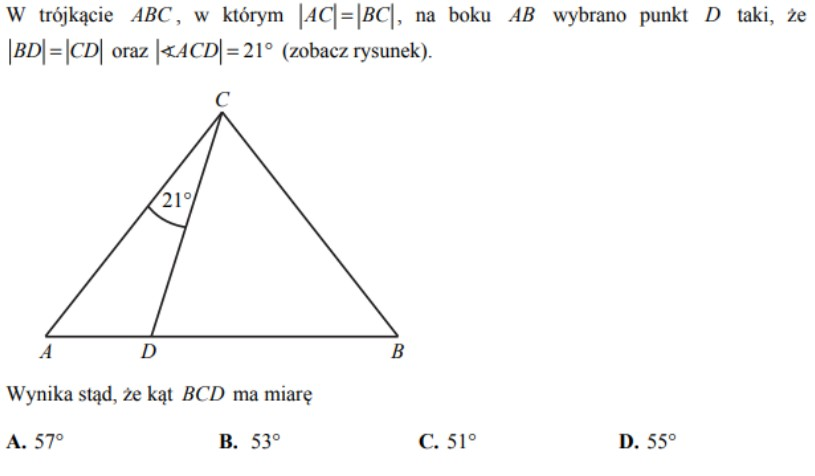
\includegraphics[scale=0.7]{z1.jpeg}
	\end{figure}
	\begin{zad}
	\end{zad}
	\begin{figure}[h]
		\centering
		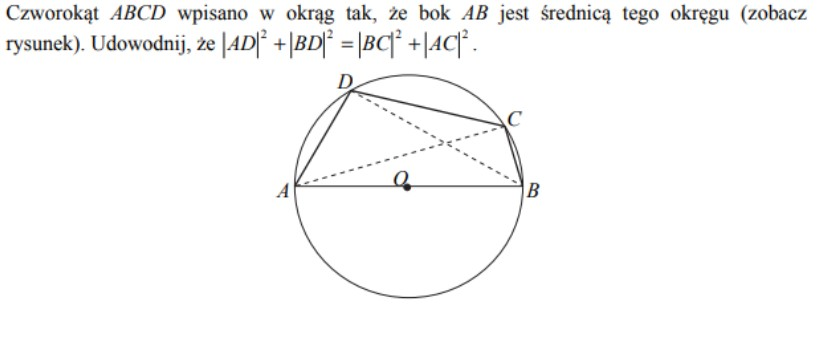
\includegraphics[scale=0.7]{z2.jpeg}
	\end{figure}	
	\begin{zad}
		Wyznacz parametr "k", dla którego trójwyrazowy ciąg
		$$(k+5,\quad k^2+4, \quad k^2+3k)$$
		jest ciągiem arytmetycznym. 
	\end{zad}
	\begin{zad}
		Oblicz sumę wszystkich liczb 3-cyfrowych podzielnych przez 4.
	\end{zad}
	\begin{zad}
		Wiedząc, że ciąg $a_n$ jest ciągiem geometrycznym. oraz że $a_4=6$ i $a_5=18$ oblicz: $q,a_1,a_{10}$.
	\end{zad}

	\begin{zad}
		 Poniżej przedstawiono interpretację geometryczną w postaci przedziału pewnej nierówności:
	\end{zad}
	
	\begin{figure}[h]
		\centering
		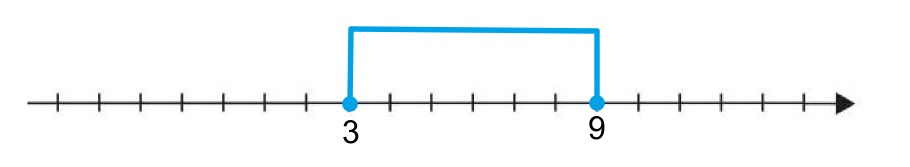
\includegraphics[scale=0.5]{z1_1.jpeg}
	\end{figure}
	
	Nierówność opisującą ten przedział można opisać za pomocą:
	
	\vspace{0.5cm}
	\begin{tabular}{p{5cm} p{5cm}}
		\textbf{A. }$|x+6|\leq3$&
		\textbf{B. }$|x-6|\leq3$\\
		\textbf{C. }$|x+6|\geq3$&
		\textbf{D. }$|x-6|\geq3$\\
	\end{tabular}
	\begin{zad}
		Usuń niewymierność z wyrażenia:
		$$\frac{1}{\sqrt{2}-1}$$
	\end{zad}
\end{document}